\documentclass{beamer}

\usefonttheme{serif}

\setbeamertemplate{footline}[frame number]{}
\setbeamertemplate{navigation symbols}{}

\usecolortheme{default}
%\setbeamercolor{block title}{bg=lily,fg=black}
%\setbeamercolor{block body}{bg = blue!10, fg = black}
\setbeamertemplate{itemize item}[square]
\setbeamercolor{itemize item}{fg = cyan}
\setbeamercolor{enumerate item}{fg = cyan}

\usetheme{default}

%\setbeamercolor{titlelike}{fg=cyan}
%Information to be included in the title page:
\title{Sample title}
\author{Anonymous}
\institute{Overleaf}
\date{2021}

\title[About Beamer] %optional
{Diffraction of light by ultrasonic waves \\ (Debye-Sears effect)}

%\subtitle{A short story}

\author[Arthur, Doe] % (optional, for multiple authors)
{A.~Simankovich \and D.~Dedkov }

\institute[VFU] % (optional)
{
	Moscow Institute of Physics and Technology
}

\date[VLC 2023] % (optional)
%{Very Large Conference, April 2021}

%\logo{\includegraphics[height=1cm]{overleaf-logo}}

\begin{document}
	
	\frame{\titlepage}
	
	\begin{frame}
		\frametitle{Abstract}
		Article describes diffraction of light by ultrasonic waves in water. Theory of diffraction by ultrasonic waves is formulated. Speed of sound is evaluated using interference pattern and dark-field method. Bulk modulus of water is estimated.
		
	\end{frame}
	
		\begin{frame}[plain,c]
		
		\begin{center}
			\huge \usebeamercolor[fg]{frametitle} Introduction and Theory
		\end{center}
		
	\end{frame}
		
	
	\begin{frame}
		\frametitle{Diffraction on periodic structures}
		
		\begin{figure}
			\centering
			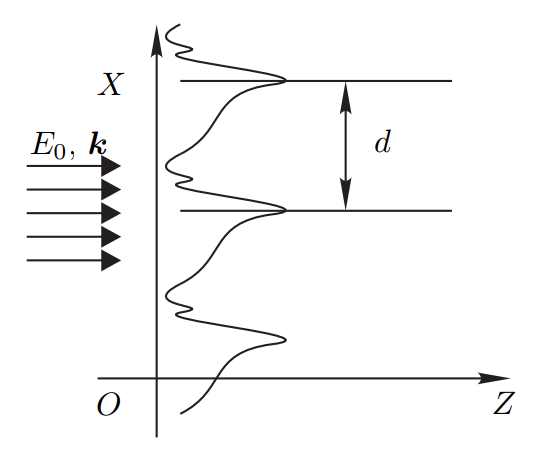
\includegraphics[width=4cm]{res/periodic.png}
			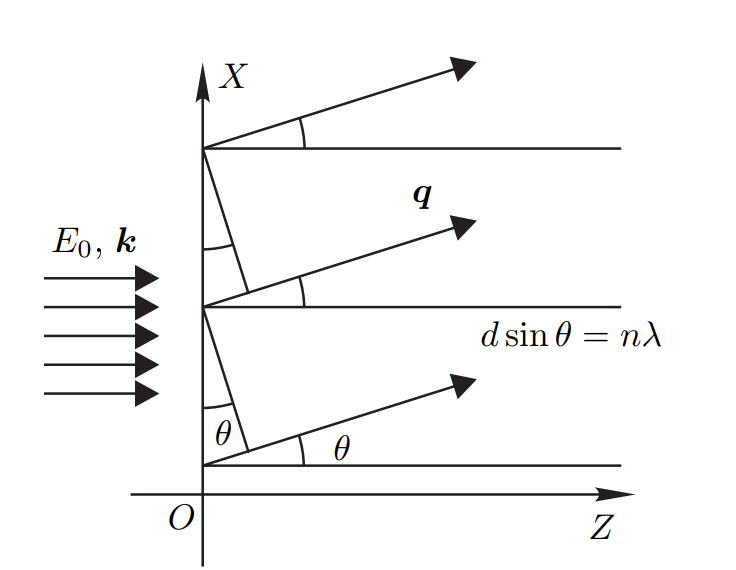
\includegraphics[width=4cm]{res/diffraction_general.png}
			\caption{Example of diffraction}
		\end{figure}
		
		
		General theory shows that when a plane light wave is normally incident on the grating, the diffracted light has maximum at diffraction angles:

		$$d \sin{\theta_m} = m \lambda,\; (m = 1, 2, ...)$$
		
	\end{frame}


	\begin{frame}
		\frametitle{Diffraction by ultrasonic waves}
		
 		\begin{figure}
			\centering
			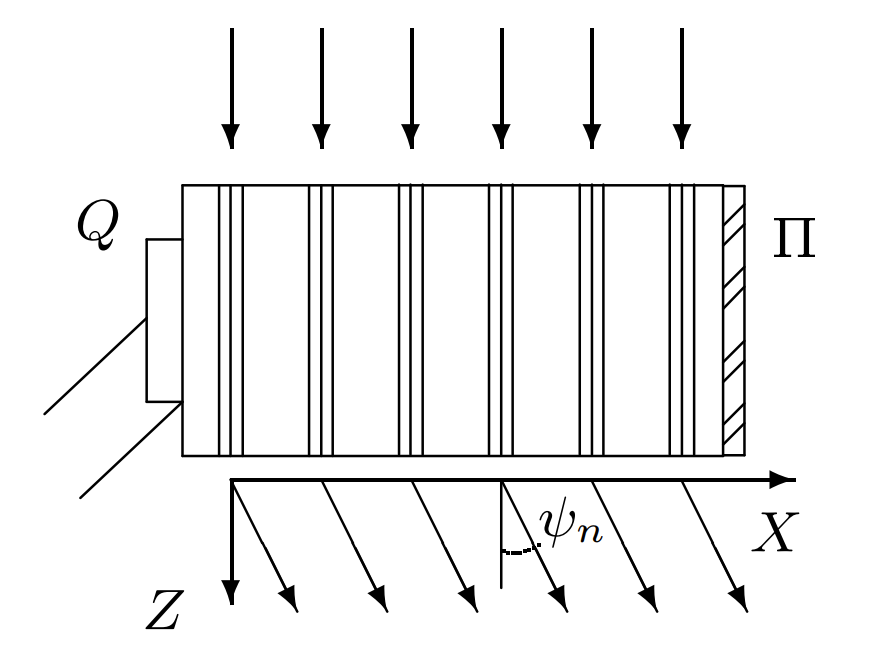
\includegraphics[width=4cm]{res/acoustic_grating.png}
			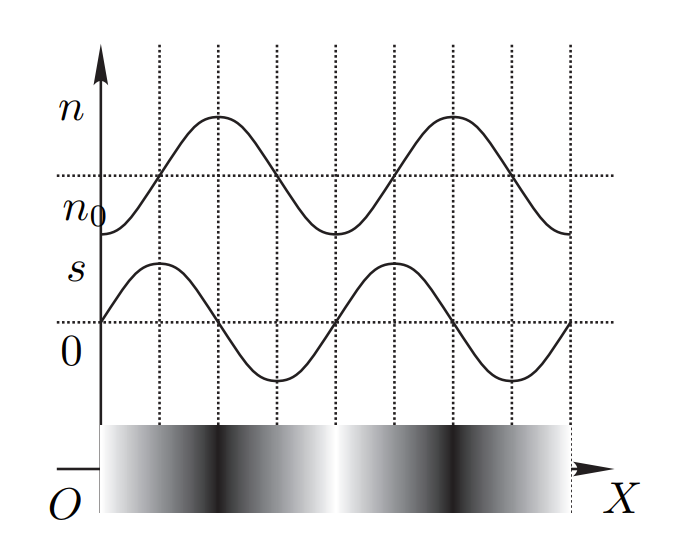
\includegraphics[width=4cm]{res/n_x.png}
			\vspace{-10pt}
			\caption{Characteristic picture of phase grating}
		\end{figure}
		One example of such system is \textbf{ultrasonic waves grating}. 
		Acoustic waves in liquids cause density changes with spacing determined by the
		frequency and the speed of the sound wave.
		Local changes in the water density lead to a change in the refractive index $n \approx n_0 (1 + a\cos{\frac{2\pi}{\Lambda}x})$, where $\Lambda$ - ultrasonic wave length.
	
		This forms a \textbf{phase diffraction grating}:
		
		\vspace{-8pt}
		\begin{equation}
			\varphi(x) = knL = \varphi_0 (1 + a \cos{\frac{2\pi}{\Lambda}x}).
			\label{eq:diffraction}
		\end{equation}
	\end{frame}

	
	\begin{frame}
		\frametitle{Velocity of the ultrasonic wave}
		
		If $\nu$ is the frequency of the ultrasonic wave, it's speed $v$ in the
		liquid is given by:
		\begin{equation}
			v = \nu \Lambda.
			\label{eq:vel}
		\end{equation}
		
		Thus, by measuring the angle of diffraction $\theta_n$, the order of diffraction $n$, the
		light wavelength, the length of ultrasonic wave in the liquid can be determined
		and then, knowing the frequency of sound wave, its speed $v$ can be obtained.
		
		Also we can deduce bulk modulus $K = \frac{\Delta P}{\Delta V / V}$:
		\begin{equation}
			K = \rho v^2.
			\label{eq:k}
		\end{equation}
	\end{frame}

	\begin{frame}
		\frametitle{Phase grating spatial structure observation}
		
				Observation of the spatial structure of the phase grating is complicated. The central problem is that phase grating intensity is \textbf{constant}. Indeed, complex transmittance has the following form:
				$$t(x) = e^{i\varphi(x)},$$ with intensity
				$$I(x) = |f_0(x)|^2 = 1.$$
				
				However, a few methods exist that allow you to observe the spatial structure.

	\end{frame}

	\begin{frame}
		\frametitle{Dark-field method}
		
		One of the most popular methods is called \textbf{dark-field method}. The idea behind is filtering the central maximum with small screen. After filtering we get:
		
		\begin{equation*}
				f_0(x) = e^{i m \cos{\Omega x}} \approx 1 +  i m \cos{\Omega x} \overset{\textbf{filtering}}{=}  i m \cos{\Omega x}.
		\end{equation*}
		Then the intensity of the filtered light is the following:
		
		\begin{equation*}
				I_f(x) = m^2 \cos^2{\Omega x} = \frac{m^2}{2} (1 + \cos{2 \Omega x}) \neq 1.
				\label{eq:dark_field}
		\end{equation*}
		$\cos{2 \Omega x}$ implies that distance between interference lines is half of grating period.
	
	\end{frame}

	\begin{frame}
		\frametitle{Phase and Amplitude Grating with Uniform Beam}
		
		\begin{figure}
			\centering
			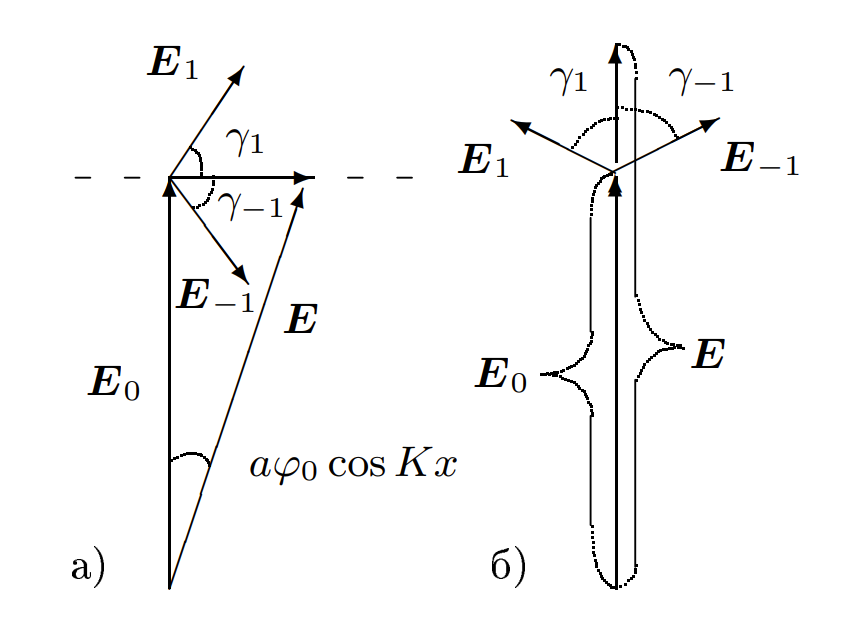
\includegraphics[width=0.5\linewidth]{res/amplitude_phase_grating}
			\caption{Phase (a) and amplitude (b) grating vector diagrams}
			\label{fig:amplitudephasegrating}
		\end{figure}
		
		The grating modulation functions are respectively ($i$ - matters):
		$$	t(x) = e^{i m \cos \Omega x} \approx 1 + \frac{im}{2}e^{i \Omega x} + \frac{im}{2}e^{-i \Omega x},$$
		
		$$	t(x) = 1 + m \cos{\Omega x} = 1 + \frac{m}{2}e^{i \Omega x} + \frac{m}{2}e^{-i \Omega x}. $$
	
	\end{frame}	

		\begin{frame}
		\frametitle{Shifting the screen}

		In other words, we can see interaction of three waves with the following modulations:
		 $1, \frac{im}{2}e^{i \Omega x},\frac{im}{2}e^{-i \Omega x}$. This gives the following waves equations: 
		$$e^{i kz}, \frac{im}{2}e^{i k(z\cos{\psi} + x\sin{\psi})},\frac{im}{2}e^{i k(z\cos{\psi} - x\sin{\psi})} \; \left(\sin{\psi} = \pm\frac{\Omega}{k}  \right)$$
		
		
		It follows from the above that there is a possibility of the phase-amplitude grating transition. Indeed, let the screen plane shift by $\Delta z$, this will result in the phase shift:
		
		$$\text{Phase shift} = k\Delta z(1 - \cos{\psi}).$$
		
		
		If $\Delta z = \frac{\pi}{2} + 2\pi n$, then the central wave $E_0$ has been rotated by $\frac{\pi}{2}$ and phase-amplitude transition has been occurred.
	\end{frame}



	\begin{frame}[plain,c]
		
		\begin{center}
			\huge \usebeamercolor[fg]{frametitle} Measurements and Results
		\end{center}
		
	\end{frame}



	\begin{frame}
		\frametitle{Experimental Setup}
		\begin{figure}
			\centering
			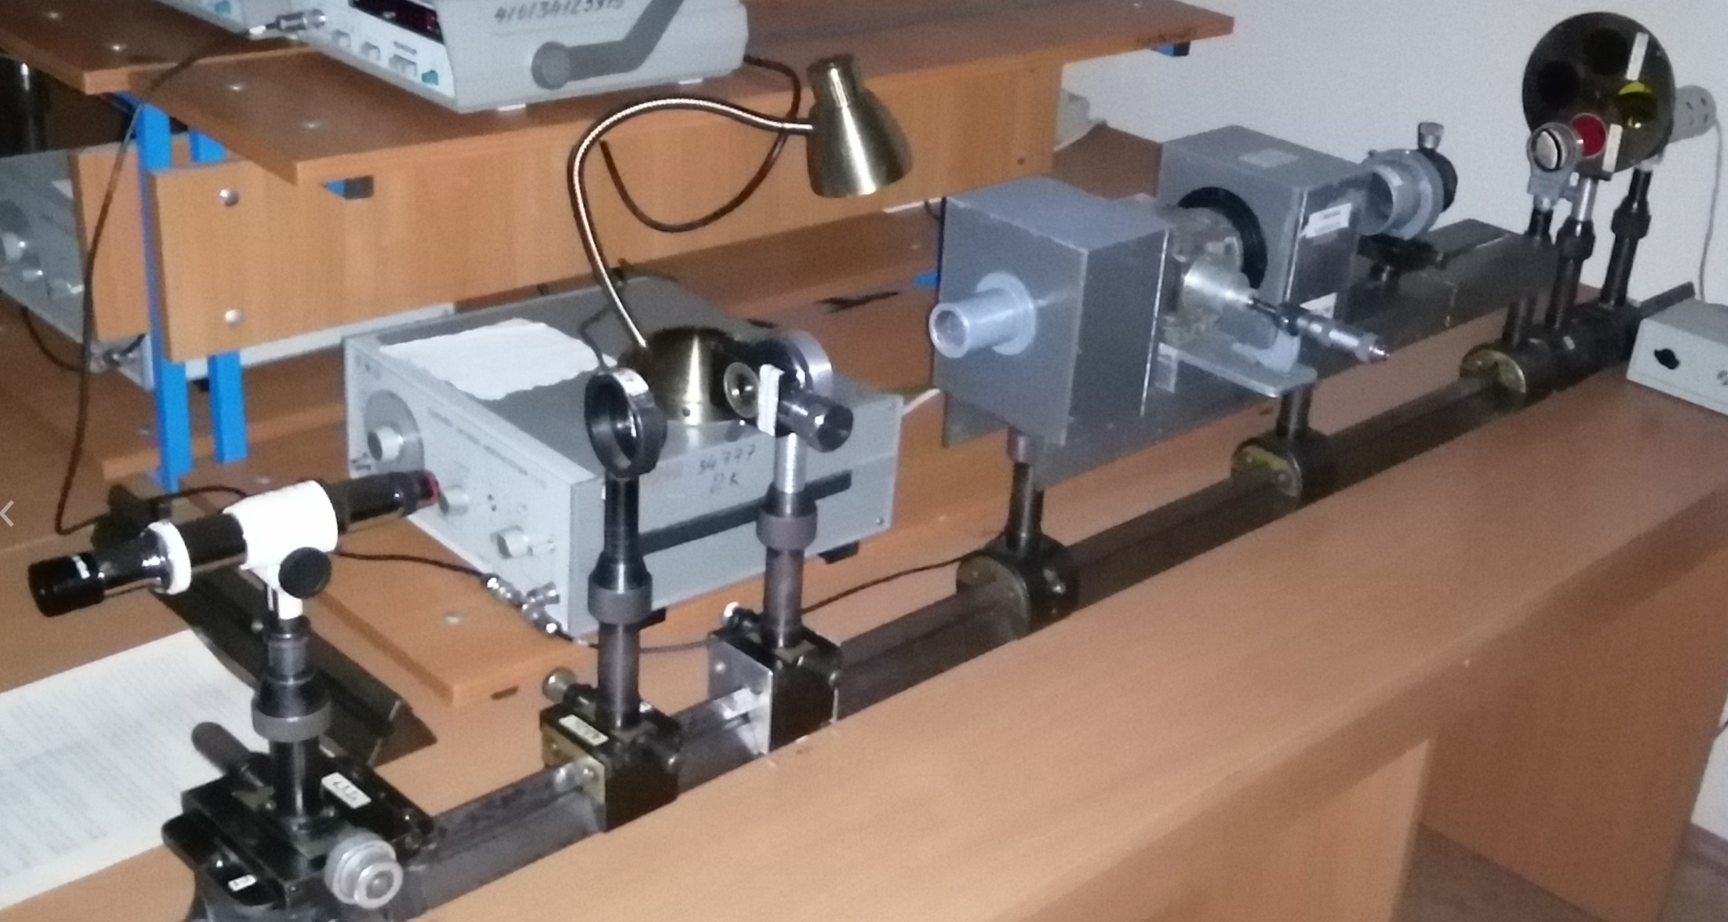
\includegraphics[width=0.8\linewidth]{res/real_setup.png}
			\caption{Photo of laboratory setup}
		\end{figure}
		
		\begin{itemize}
			\item $f = (30 \pm 0.1)$ cm -- focal length of lenses
			\item $\lambda = (640 \pm 20)$ nm -- light wave length (red)
			\item $\nu \in [1.0; 5.0]$ MHz -- ultrasonic generator frequency range
			
		\end{itemize}		
	\end{frame}
	

	\begin{frame}
		\frametitle{Experimental Setup}
		\begin{figure}
			\centering
			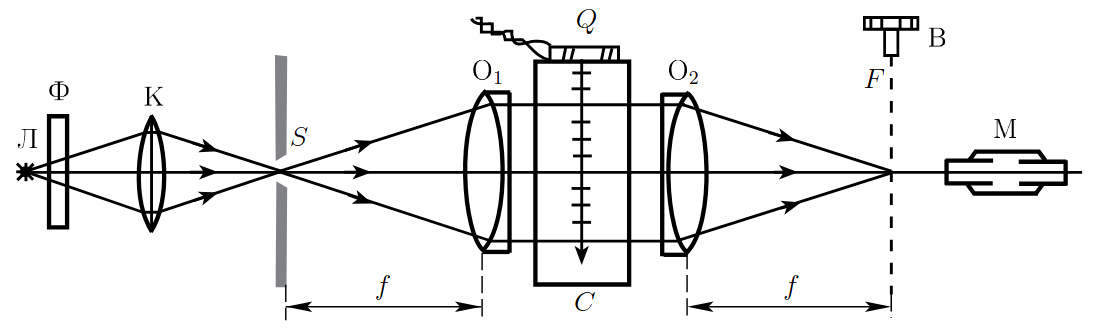
\includegraphics[width=10cm]{res/setup1.png}
		\end{figure}
		
		\begin{columns}
			\column{0.35\textwidth}
			\begin{enumerate}
				\item[$\bullet$] $L$ - light source
				\item[$\bullet$] $\Phi$ - light filter
				\item[$\bullet$] $K$ - condenser
				\item[$\bullet$] $O_1, O_2$ - lenses
				\item[$\bullet$] $Q$ - cuvette
				\item[$\bullet$] $B$ - measurement screw
				\item[$\bullet$] $M$ - microscope
			\end{enumerate}
			\column{0.70\linewidth}
			Light source $L$ illuminates slit $S$ through $\Phi$ and $K$. Parallel light beam passes through cuvette $Q$. Ultrasonic signal from generator is supplied to quartz piezoelectric plate. Light interacts with ultrasonic wave, resulting in interference pattern in focal plane of $O_2$. Pattern can be observed in microscope.
		\end{columns}
	\end{frame}
	
	\begin{frame}
		\frametitle{Observing diffraction lines}

		\begin{figure}
			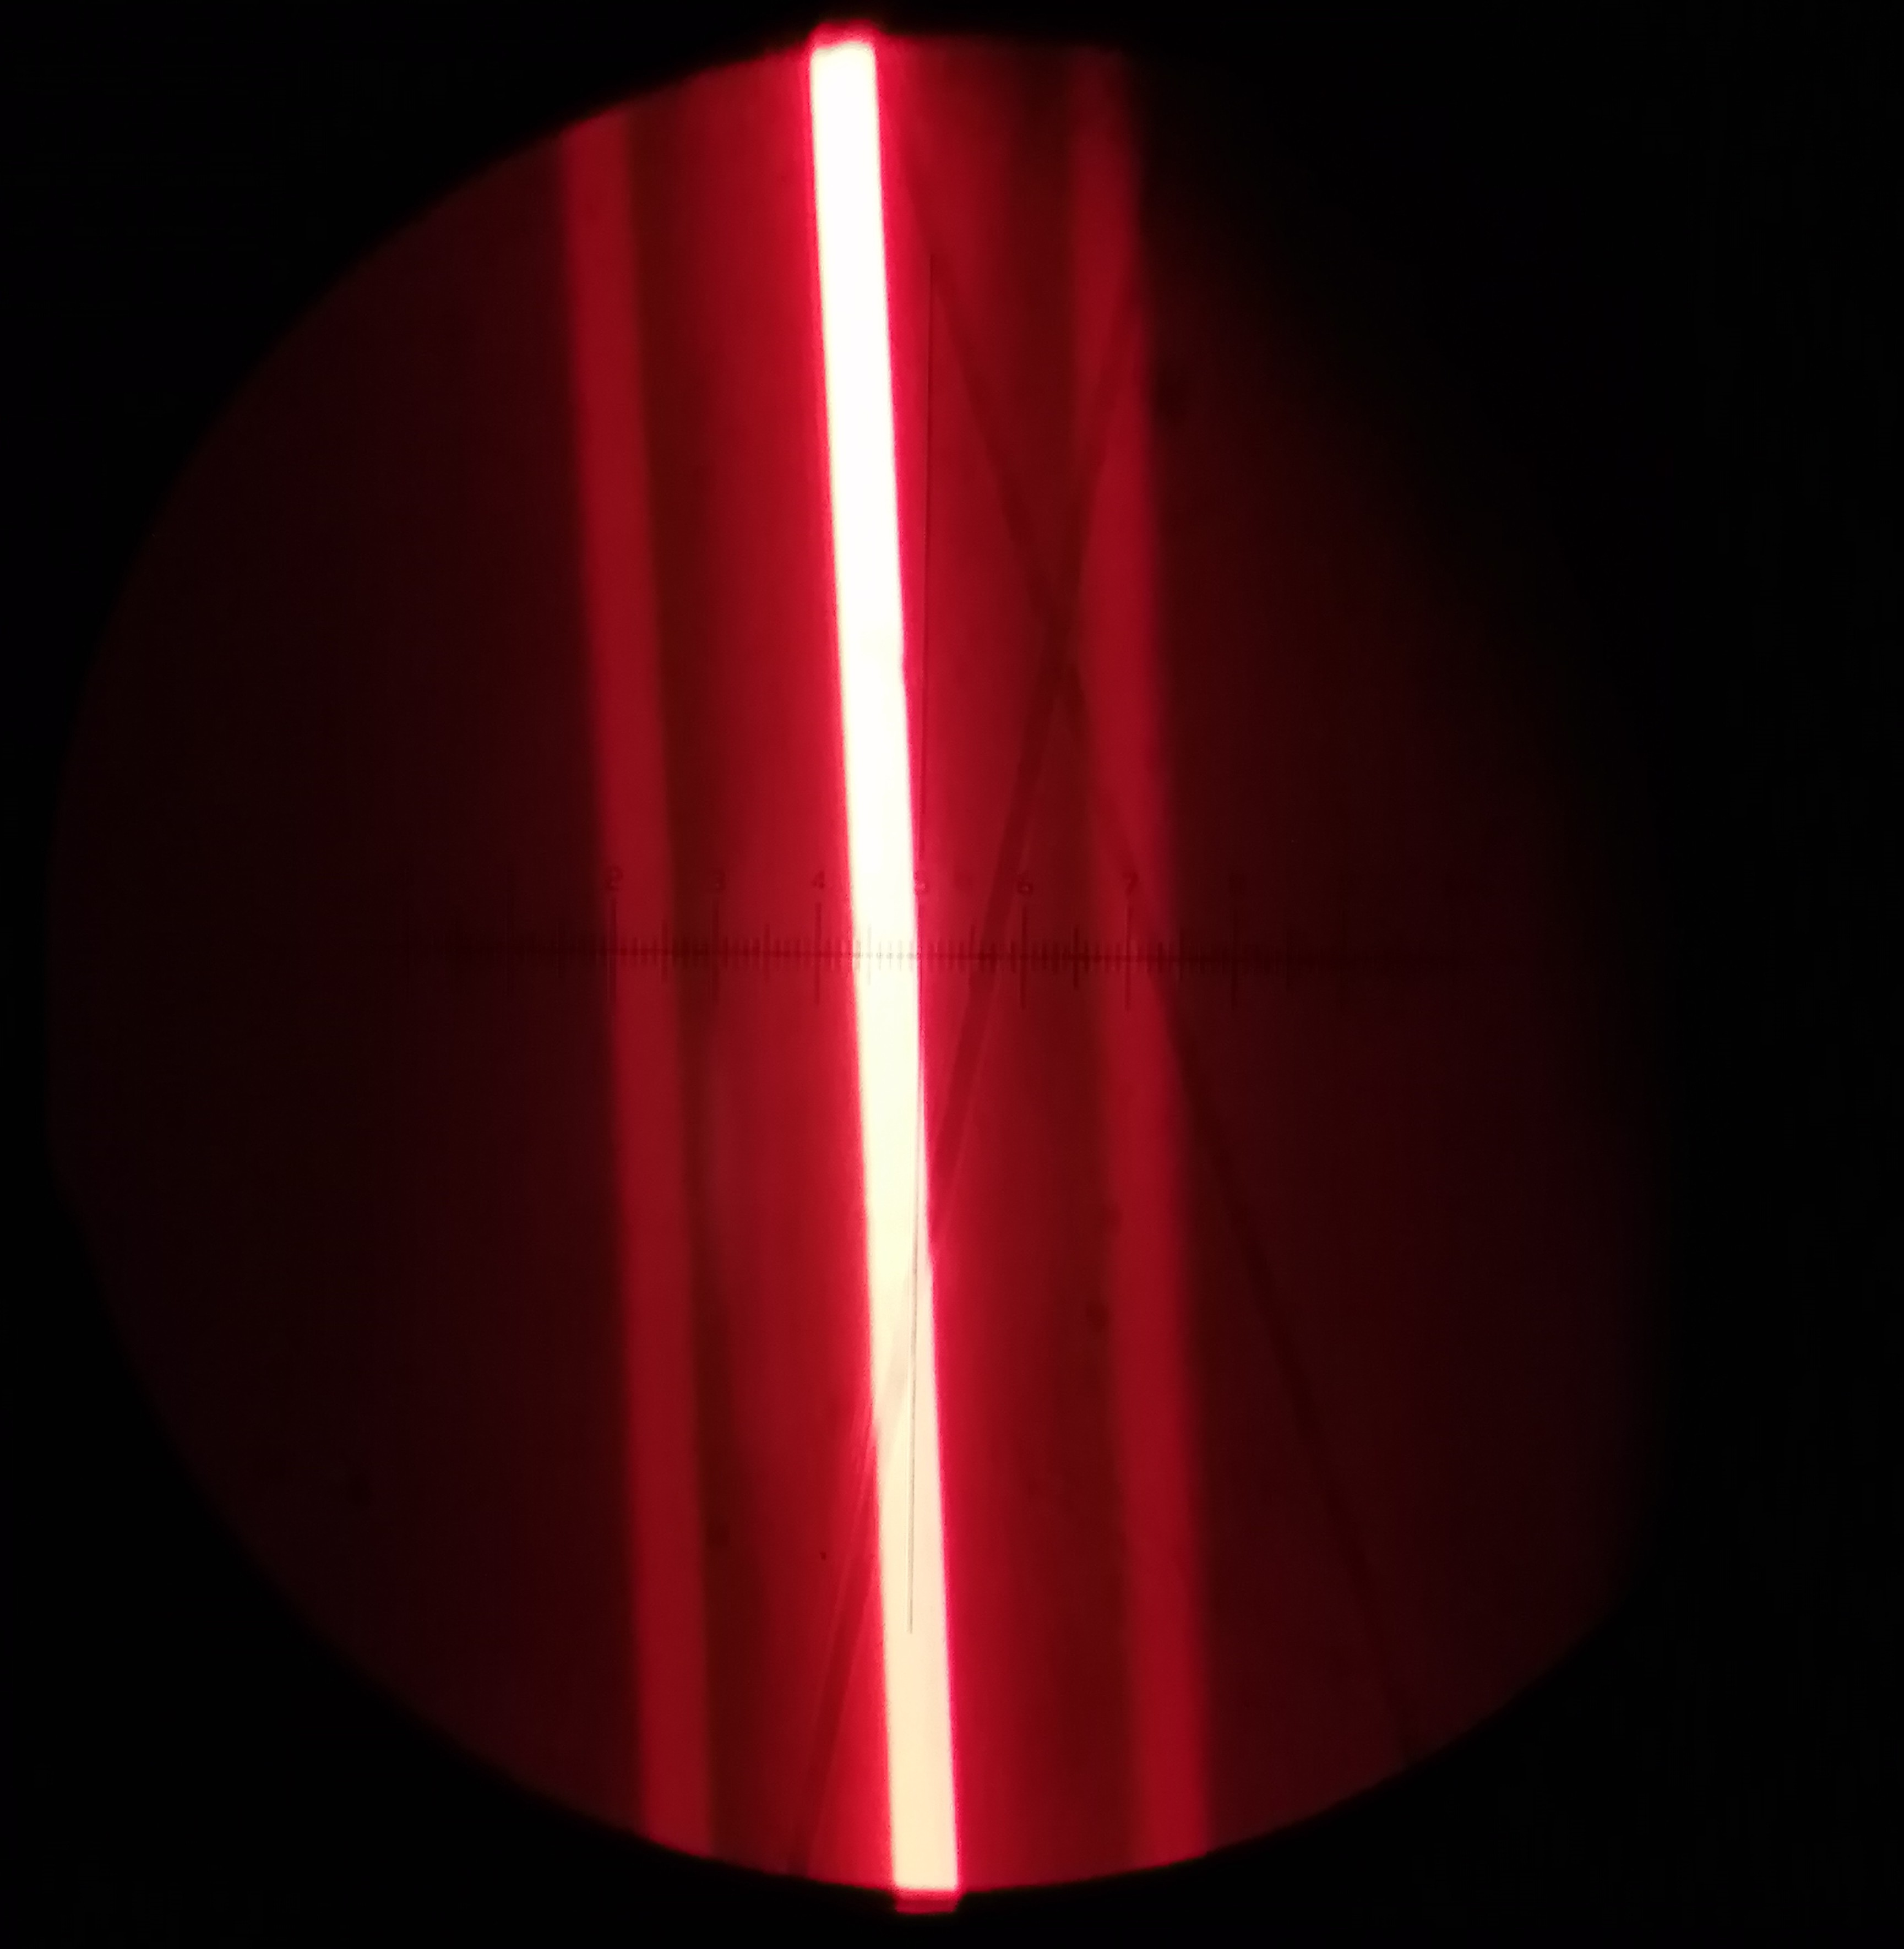
\includegraphics[height=4cm]{data/part1/1.jpg}
			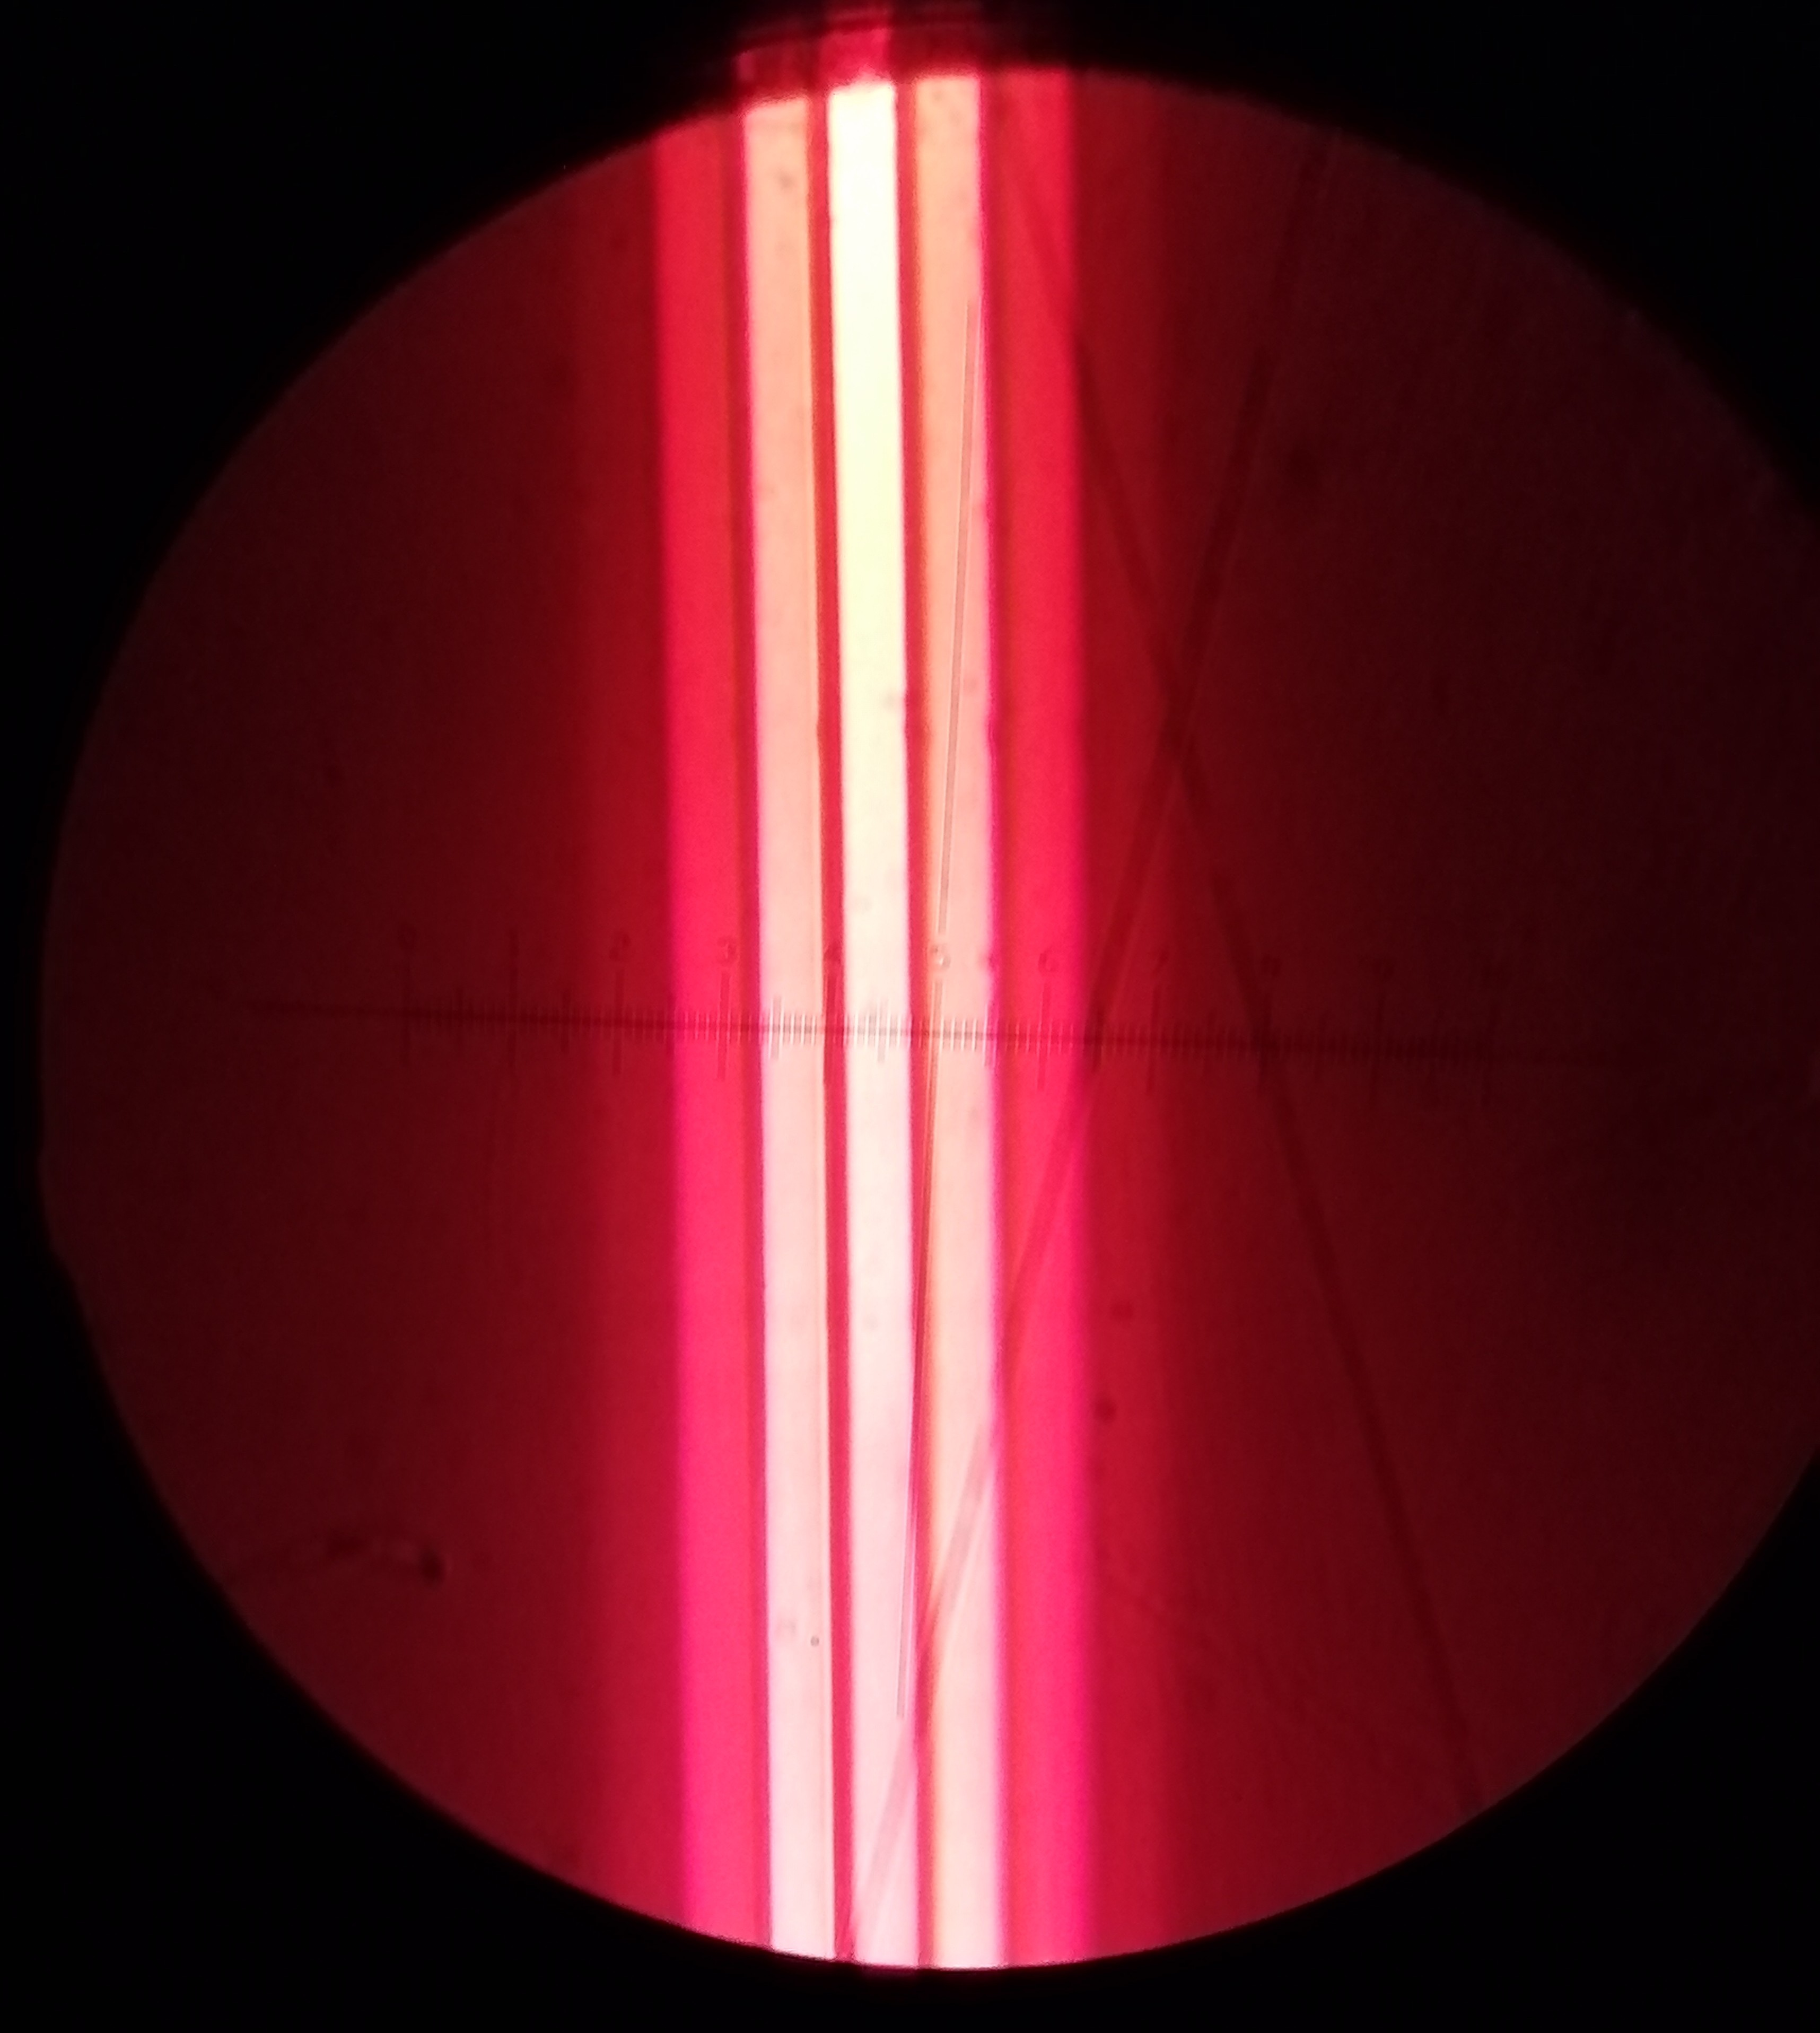
\includegraphics[height=4cm]{data/part1/2.jpg}
			\caption{Diffraction lines in microscope}
		\end{figure}
	
		\begin{columns}
			\column{0.6\textwidth}
			As described above, we can see interference pattern on different frequencies. We use glass with thin notches and measurement screw $B$ to determine distances between diffraction lines.
			\column{0.4\textwidth}
			\begin{figure}
				\centering
				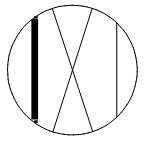
\includegraphics[width=0.5\linewidth]{res/measurement_glass.png}
				\vspace{-5pt}
				\caption{Notches scheme}
			\end{figure}
		\end{columns}
	
	\end{frame}


	\begin{frame}
		\frametitle{Cuvette length variation}

		Using screw on cuvette we can change it's length. We setup generator frequency to achive well-recognizable interference pattern ($\nu = 1.16$ MHz). In that case wave becomes standing. Taking into account that changing cuvette length to $\Lambda / 2$ again gives us standing wave, we estimate: 
		
		$$ \Lambda / 2 = (700 \pm 70)\; \text{mkm} \Rightarrow v = \Lambda \nu = (1600 \pm 160) \;\text{m/s}.$$
		
	\end{frame}


	\begin{frame}
		\frametitle{Diffraction maxima}
		\begin{columns}
			\column{0.6\textwidth}
			\begin{figure}
				\centering
				\includegraphics[width=1.1\linewidth]{gen/part1_xn.pdf}
				\caption{Maxima positions for different frequencies}
				\label{fig:part1_xn}
			\end{figure}
			\column{0.4\textwidth}
			Slope coefficient $k = \frac{dx}{dm}$.
			
			From (\ref{eq:diffraction}) and (\ref{eq:vel}):
			$$ v = \frac{f \lambda \nu m}{x_m} = \frac{f \lambda \nu}{k}.$$
			
			After evaluating $k$ for every frequency and taking average:
			$$ v = (1480 \pm 30)\; \text{m/s}.$$
			
		\end{columns}
				
	\end{frame}

	\begin{frame}
		\frametitle{Experimental Setup}
		\begin{figure}
			\centering
			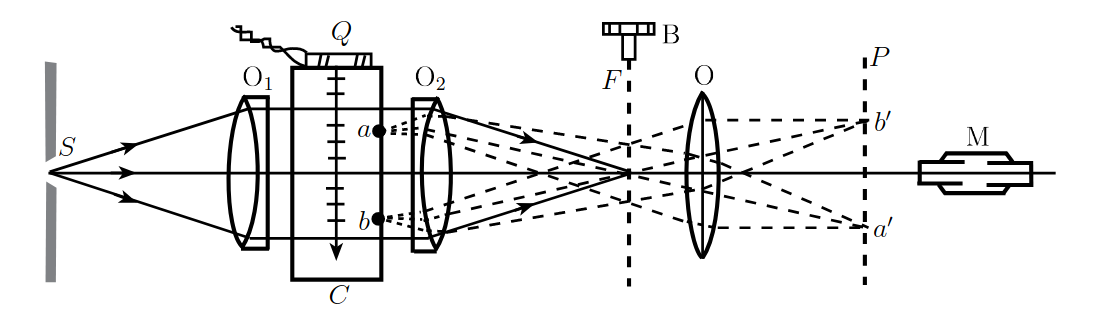
\includegraphics[width=10cm]{res/setup2.png}
		\end{figure}
		
		\begin{columns}
			\column{0.35\textwidth}
			\begin{enumerate}
				\item[$\bullet$] $S$ - slit
				\item[$\bullet$] $O_1, O_2$ - lenses
				\item[$\bullet$] $Q$ - cuvette
				\item[$\bullet$] $B$ - measurement screw
				\item[$\bullet$] $O$ - auxiliary lens
				\item[$\bullet$] $P$ - clear-image plane
				\item[$\bullet$] $M$ - microscope
			\end{enumerate}
			\column{0.70\linewidth}
			Comparing with previous setup, we add auxiliary lens $O$. It creates clear image of objects in cuvette $Q$ in plane $P$. We use wire to cut off central maximum in $O_2$ focal plane. Interference pattern can be observed in microscope.
		\end{columns}
	\end{frame}
	
	\begin{frame}
		\frametitle{Dark-field calibration}
		
		\begin{figure}
			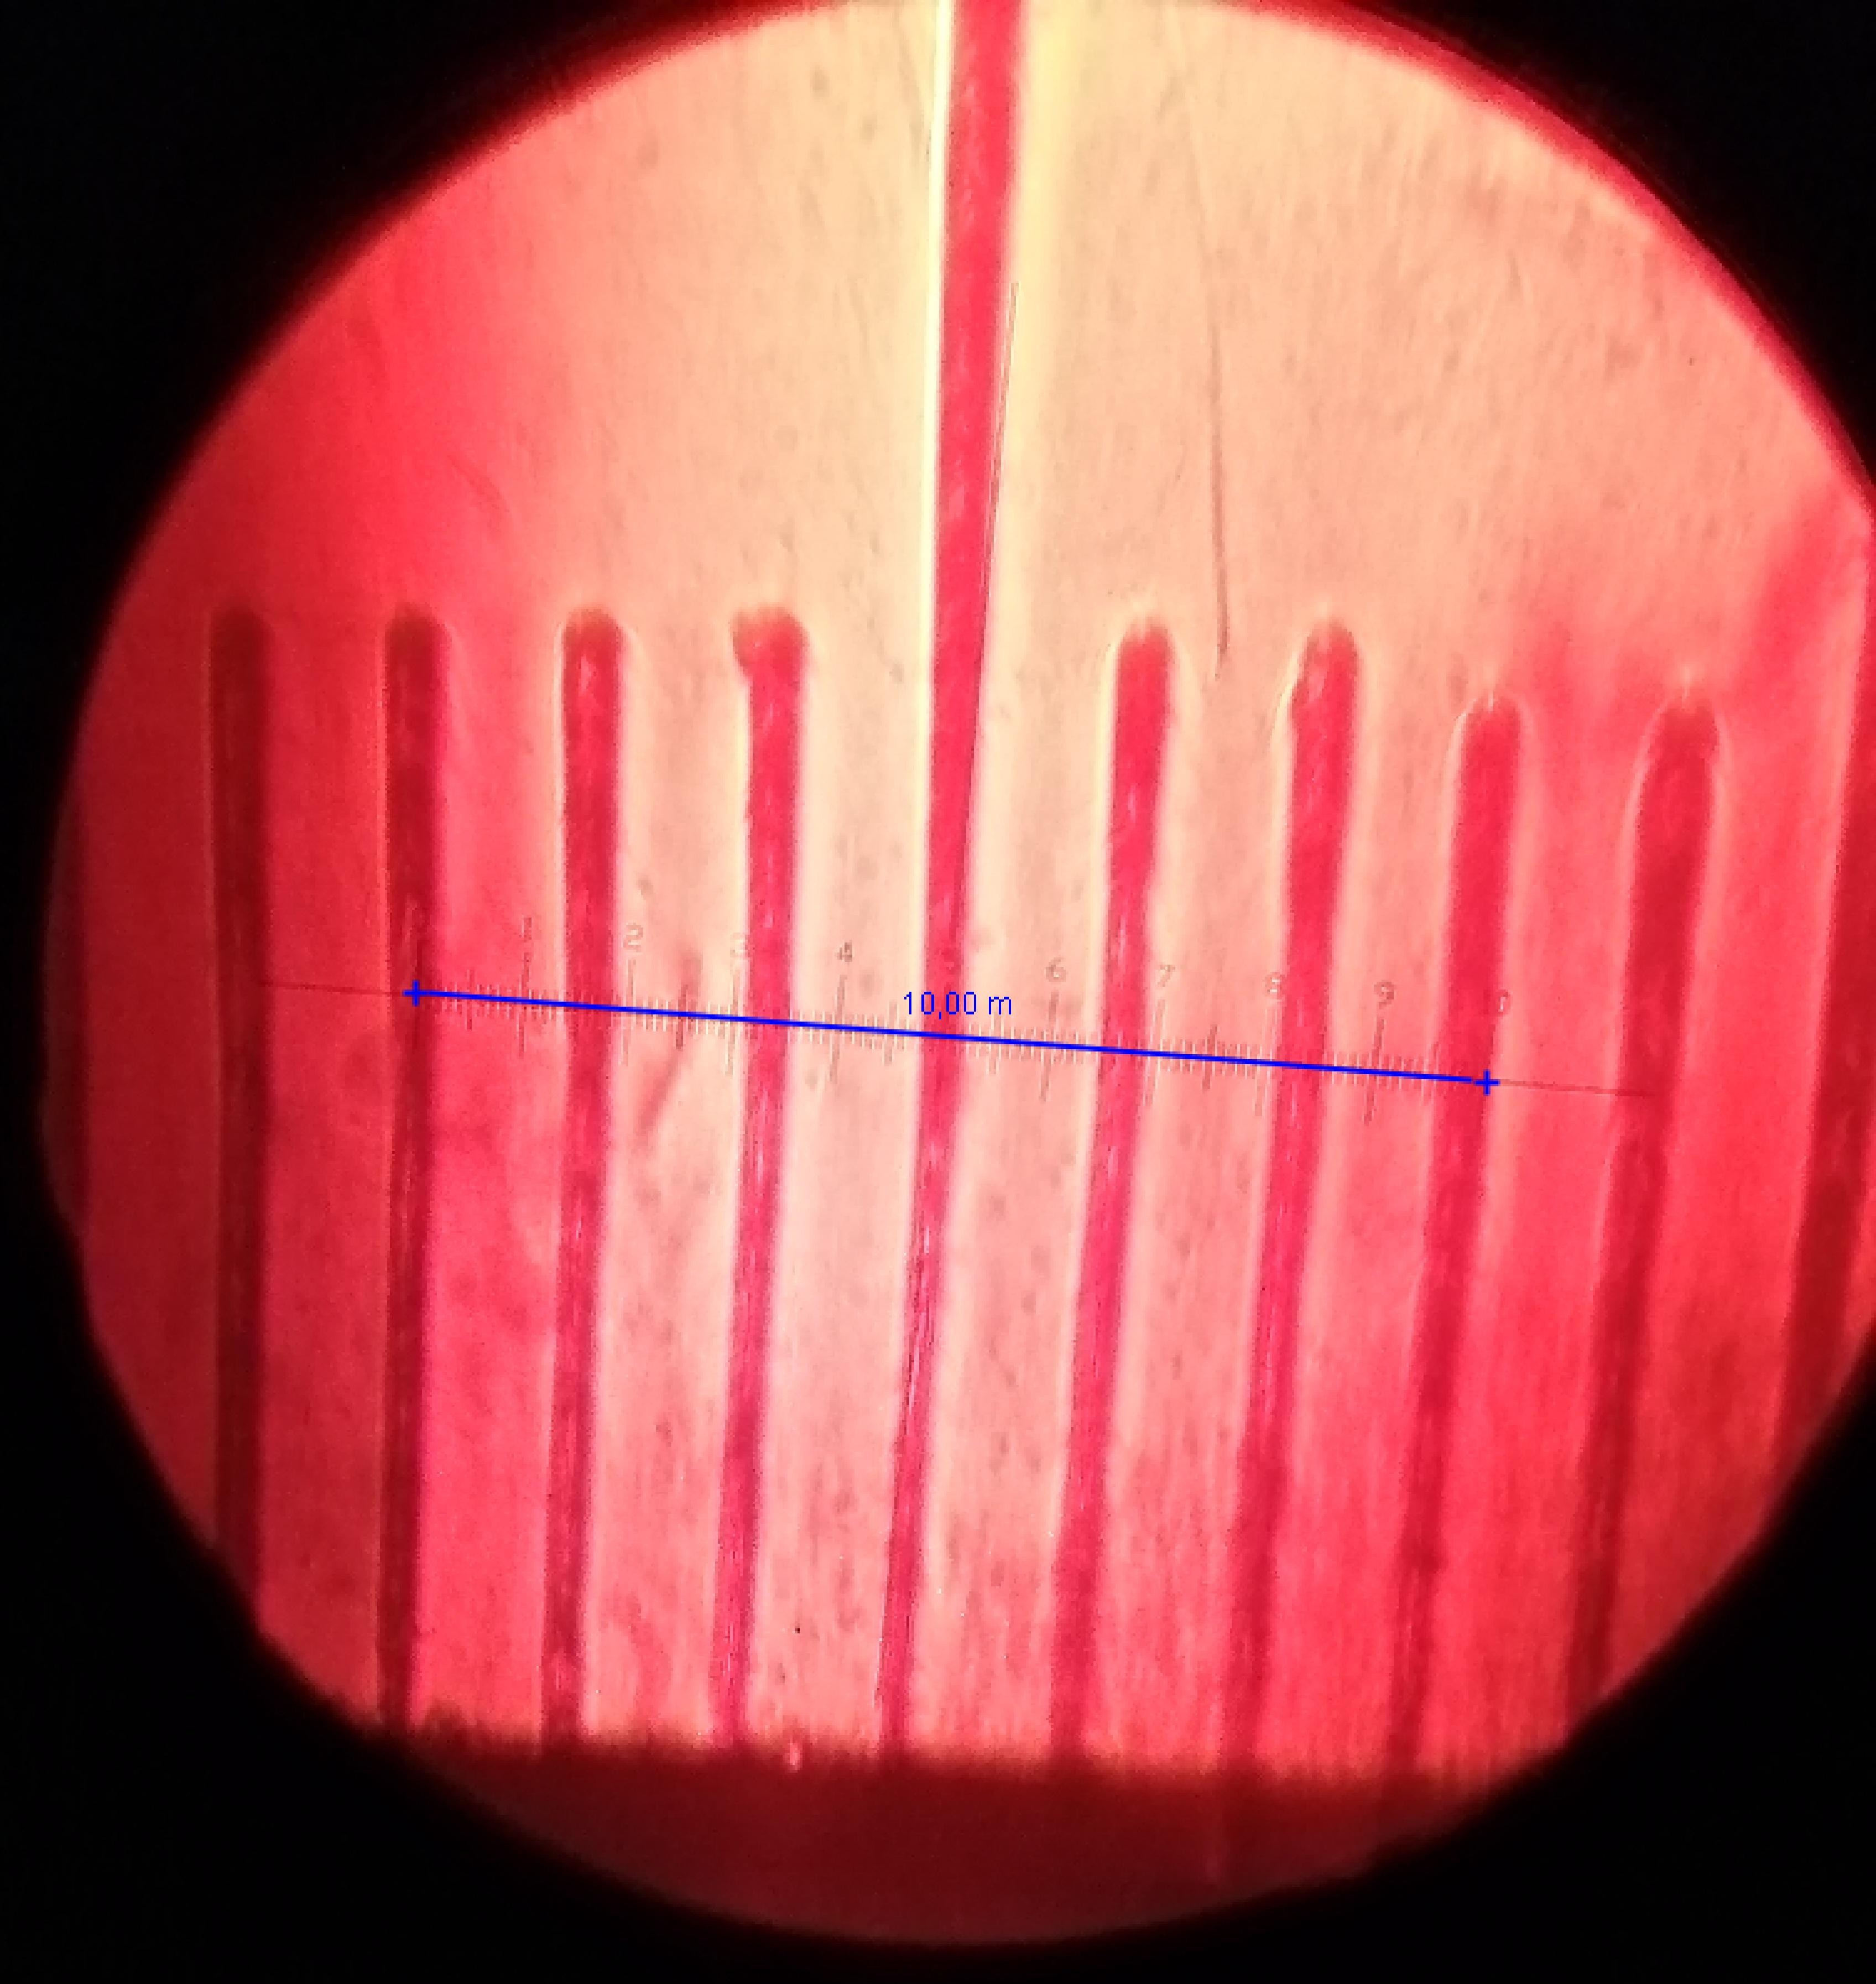
\includegraphics[width=4cm]{data/part2/ruler.jpg}
			\caption{Calibration ruler in microscope}
		\end{figure}
	
		To determine distance between interference lines we calibrate microscope scale using glass with millimeter notches. Scale coefficient $\gamma = (0.60 \pm 0.05)$ mm/div.
		
	\end{frame}
	

	\begin{frame}
		\frametitle{Observing dark-field lines}
		
		\begin{figure}
			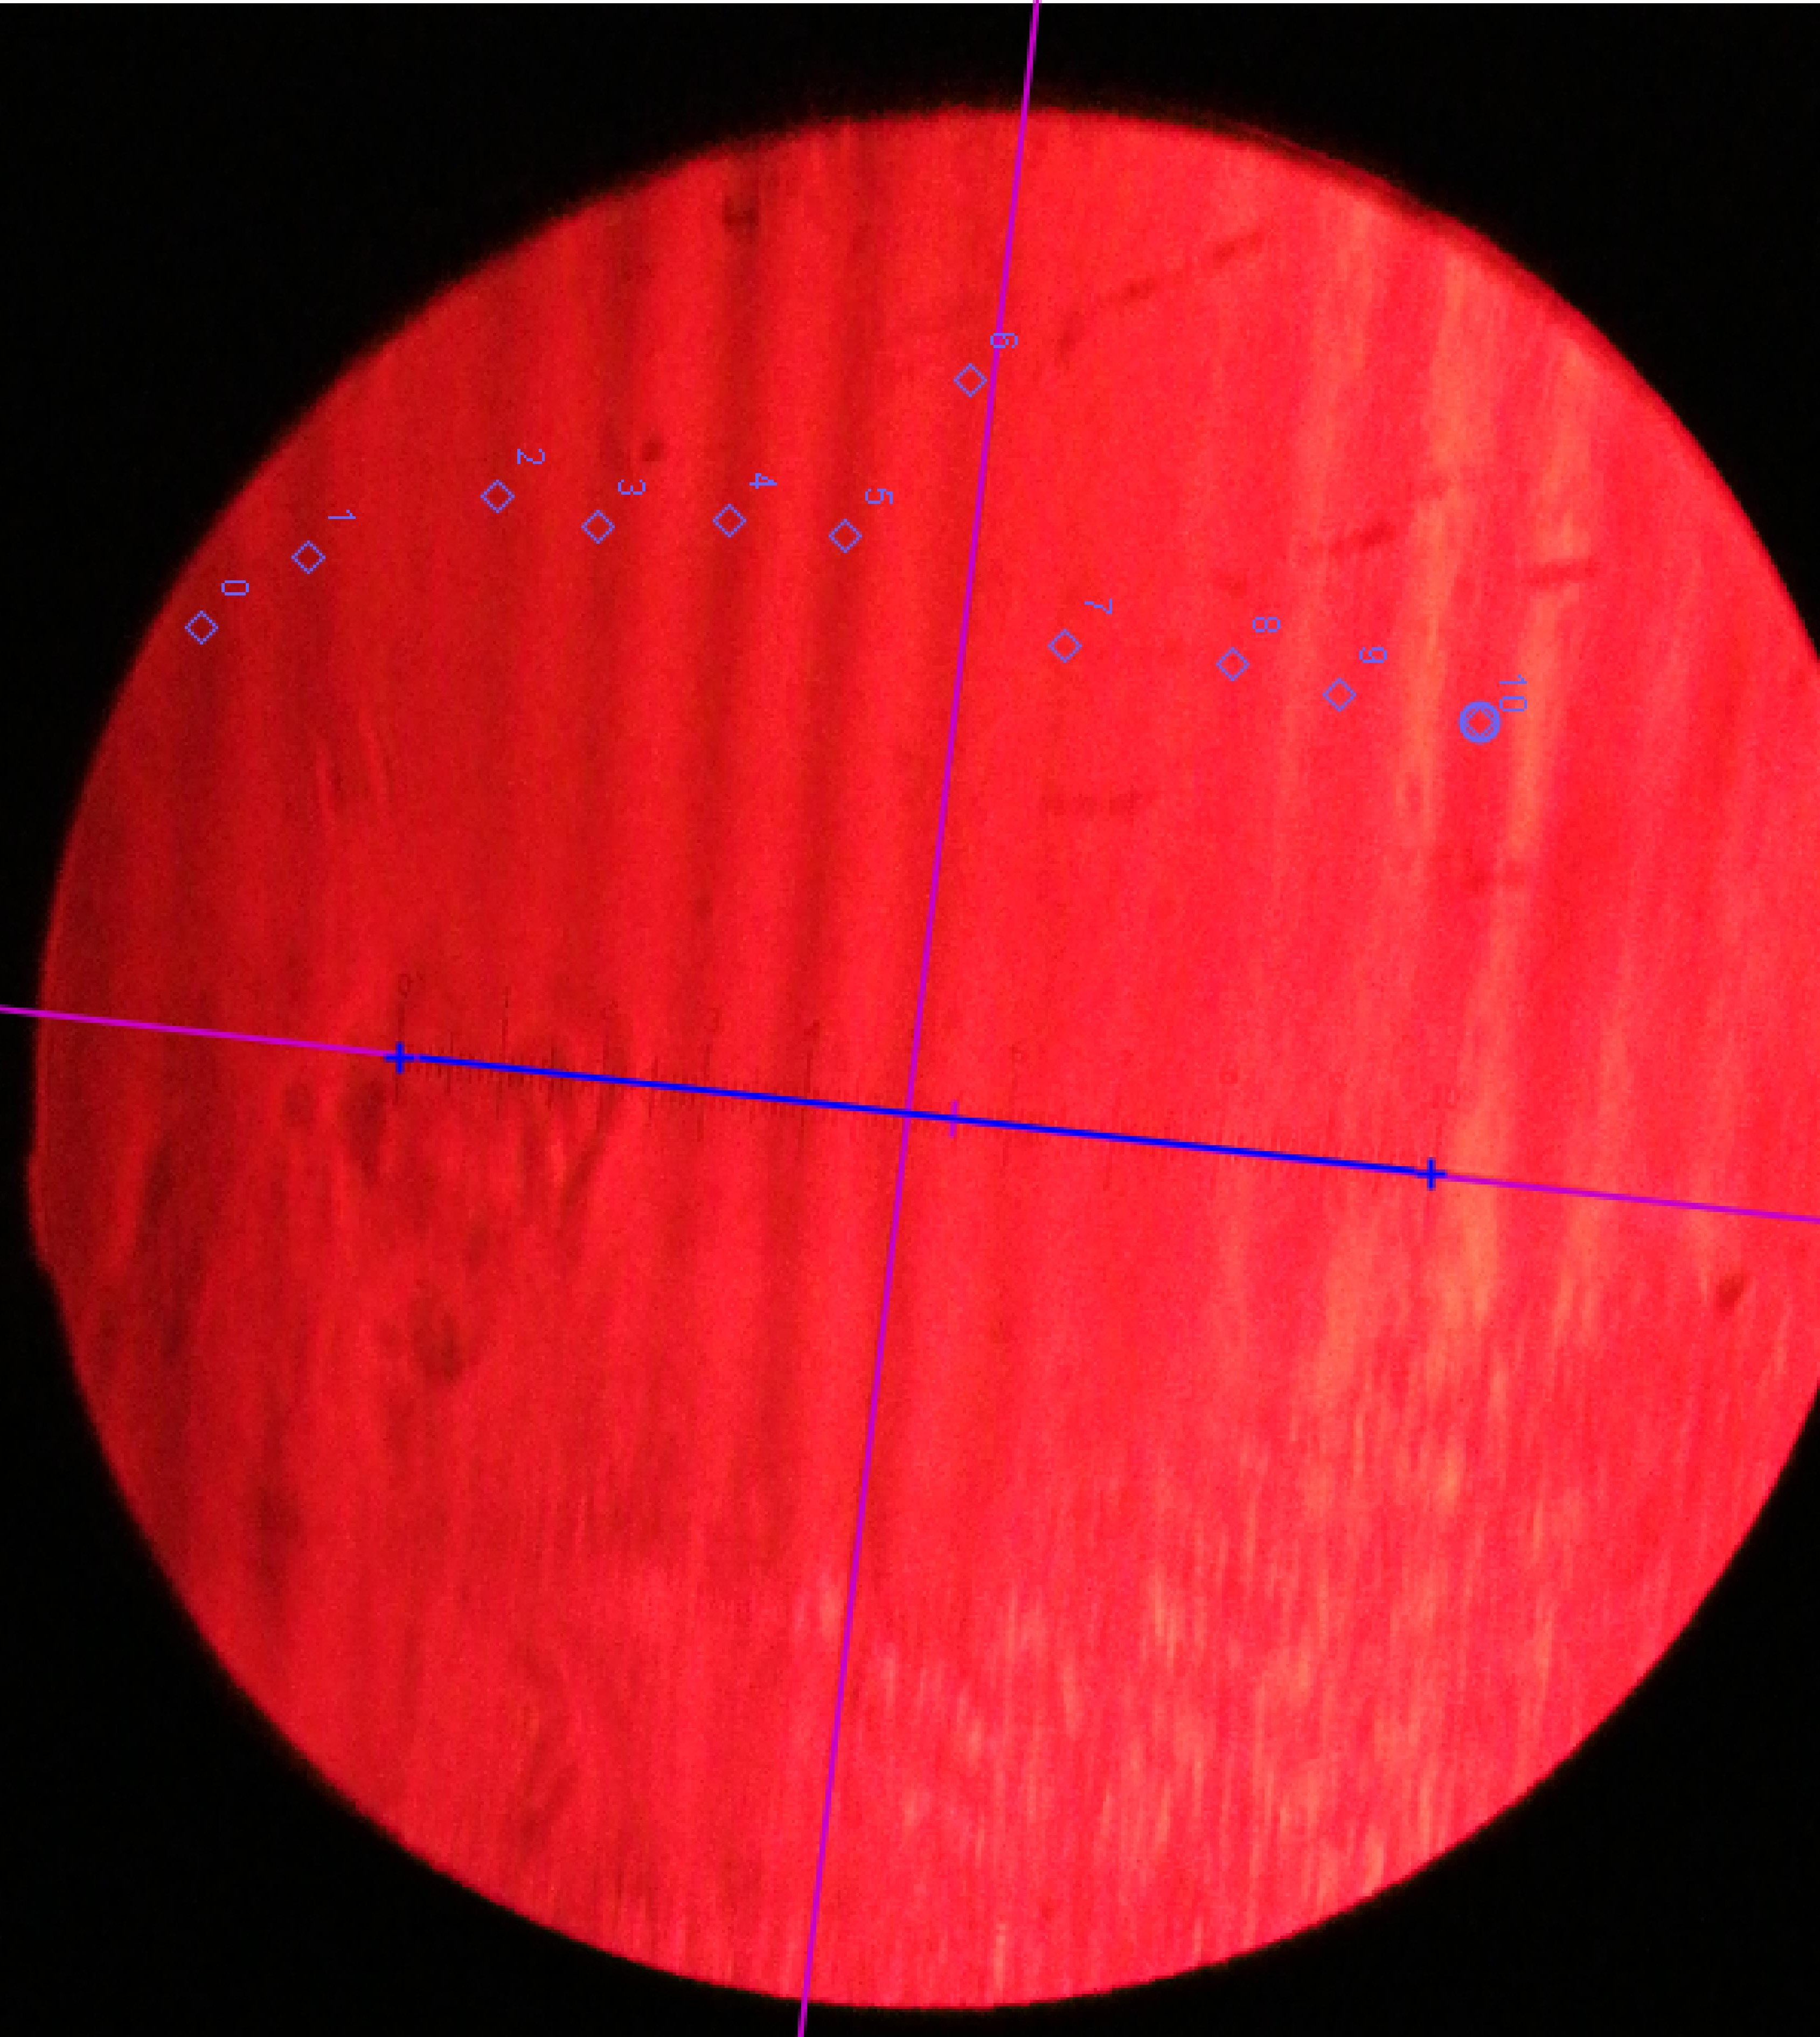
\includegraphics[height=3.5cm]{data/part2/1.jpg}
			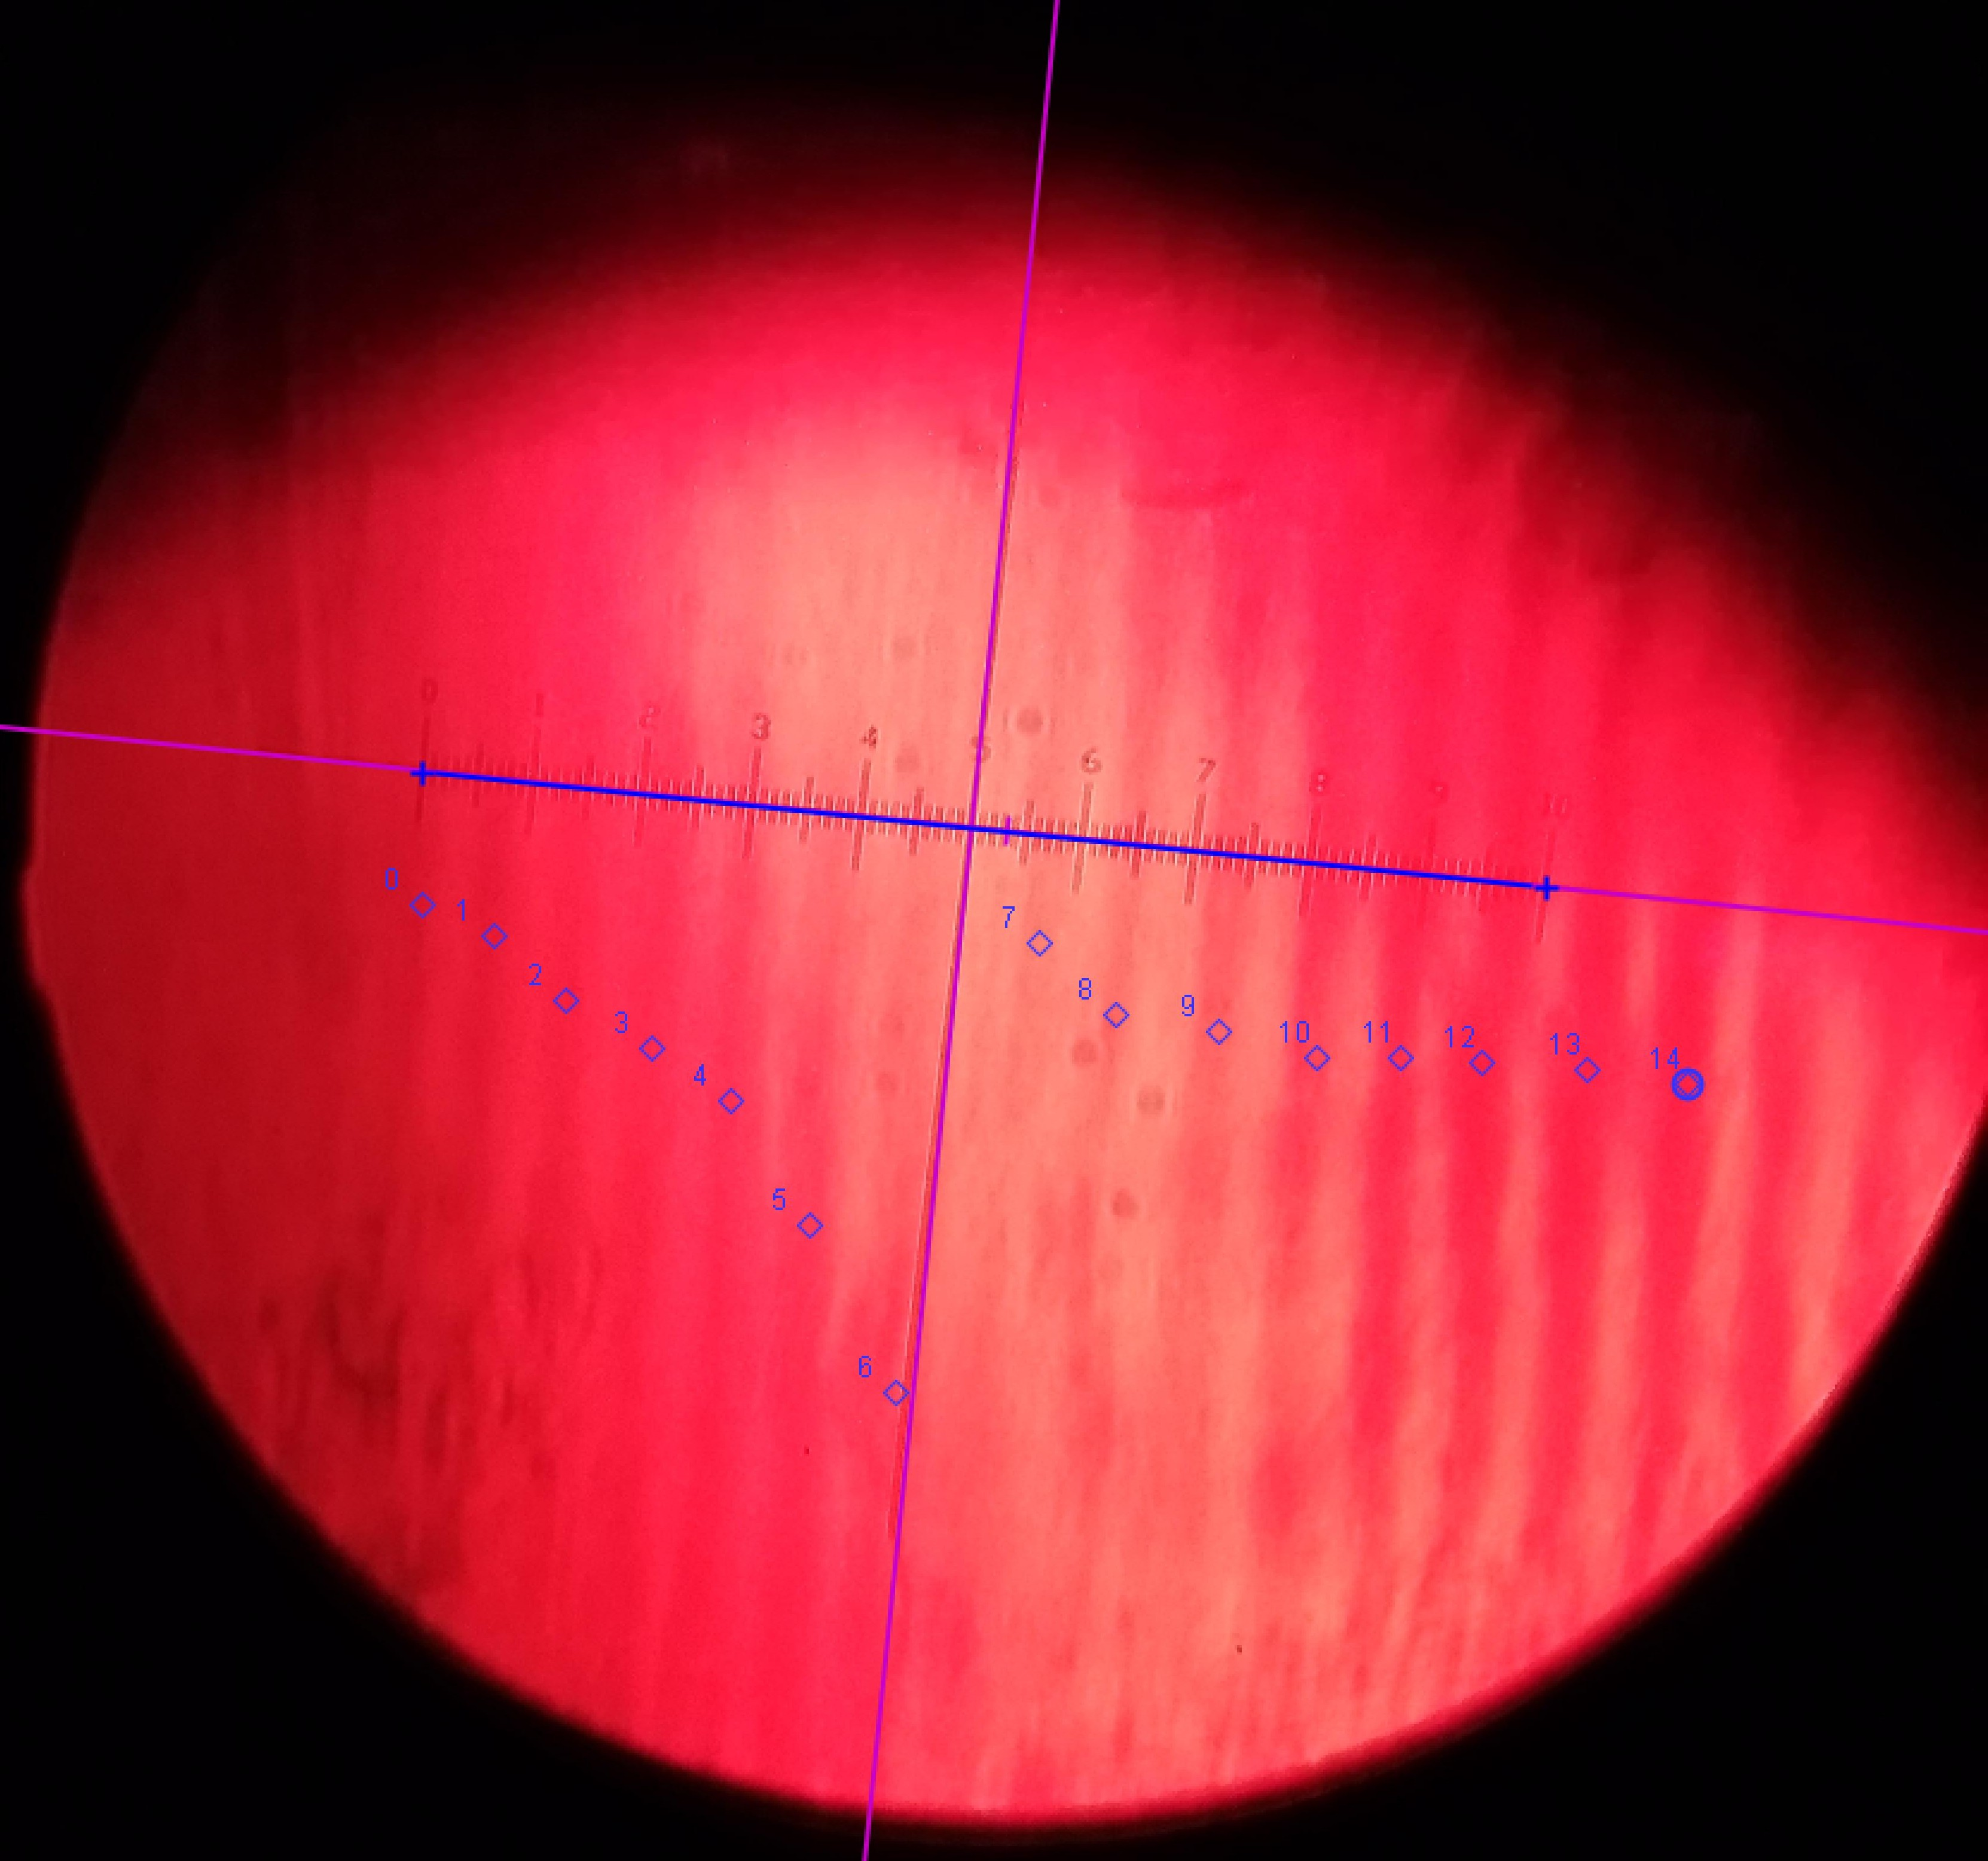
\includegraphics[height=3.5cm]{data/part2/2.jpg}
			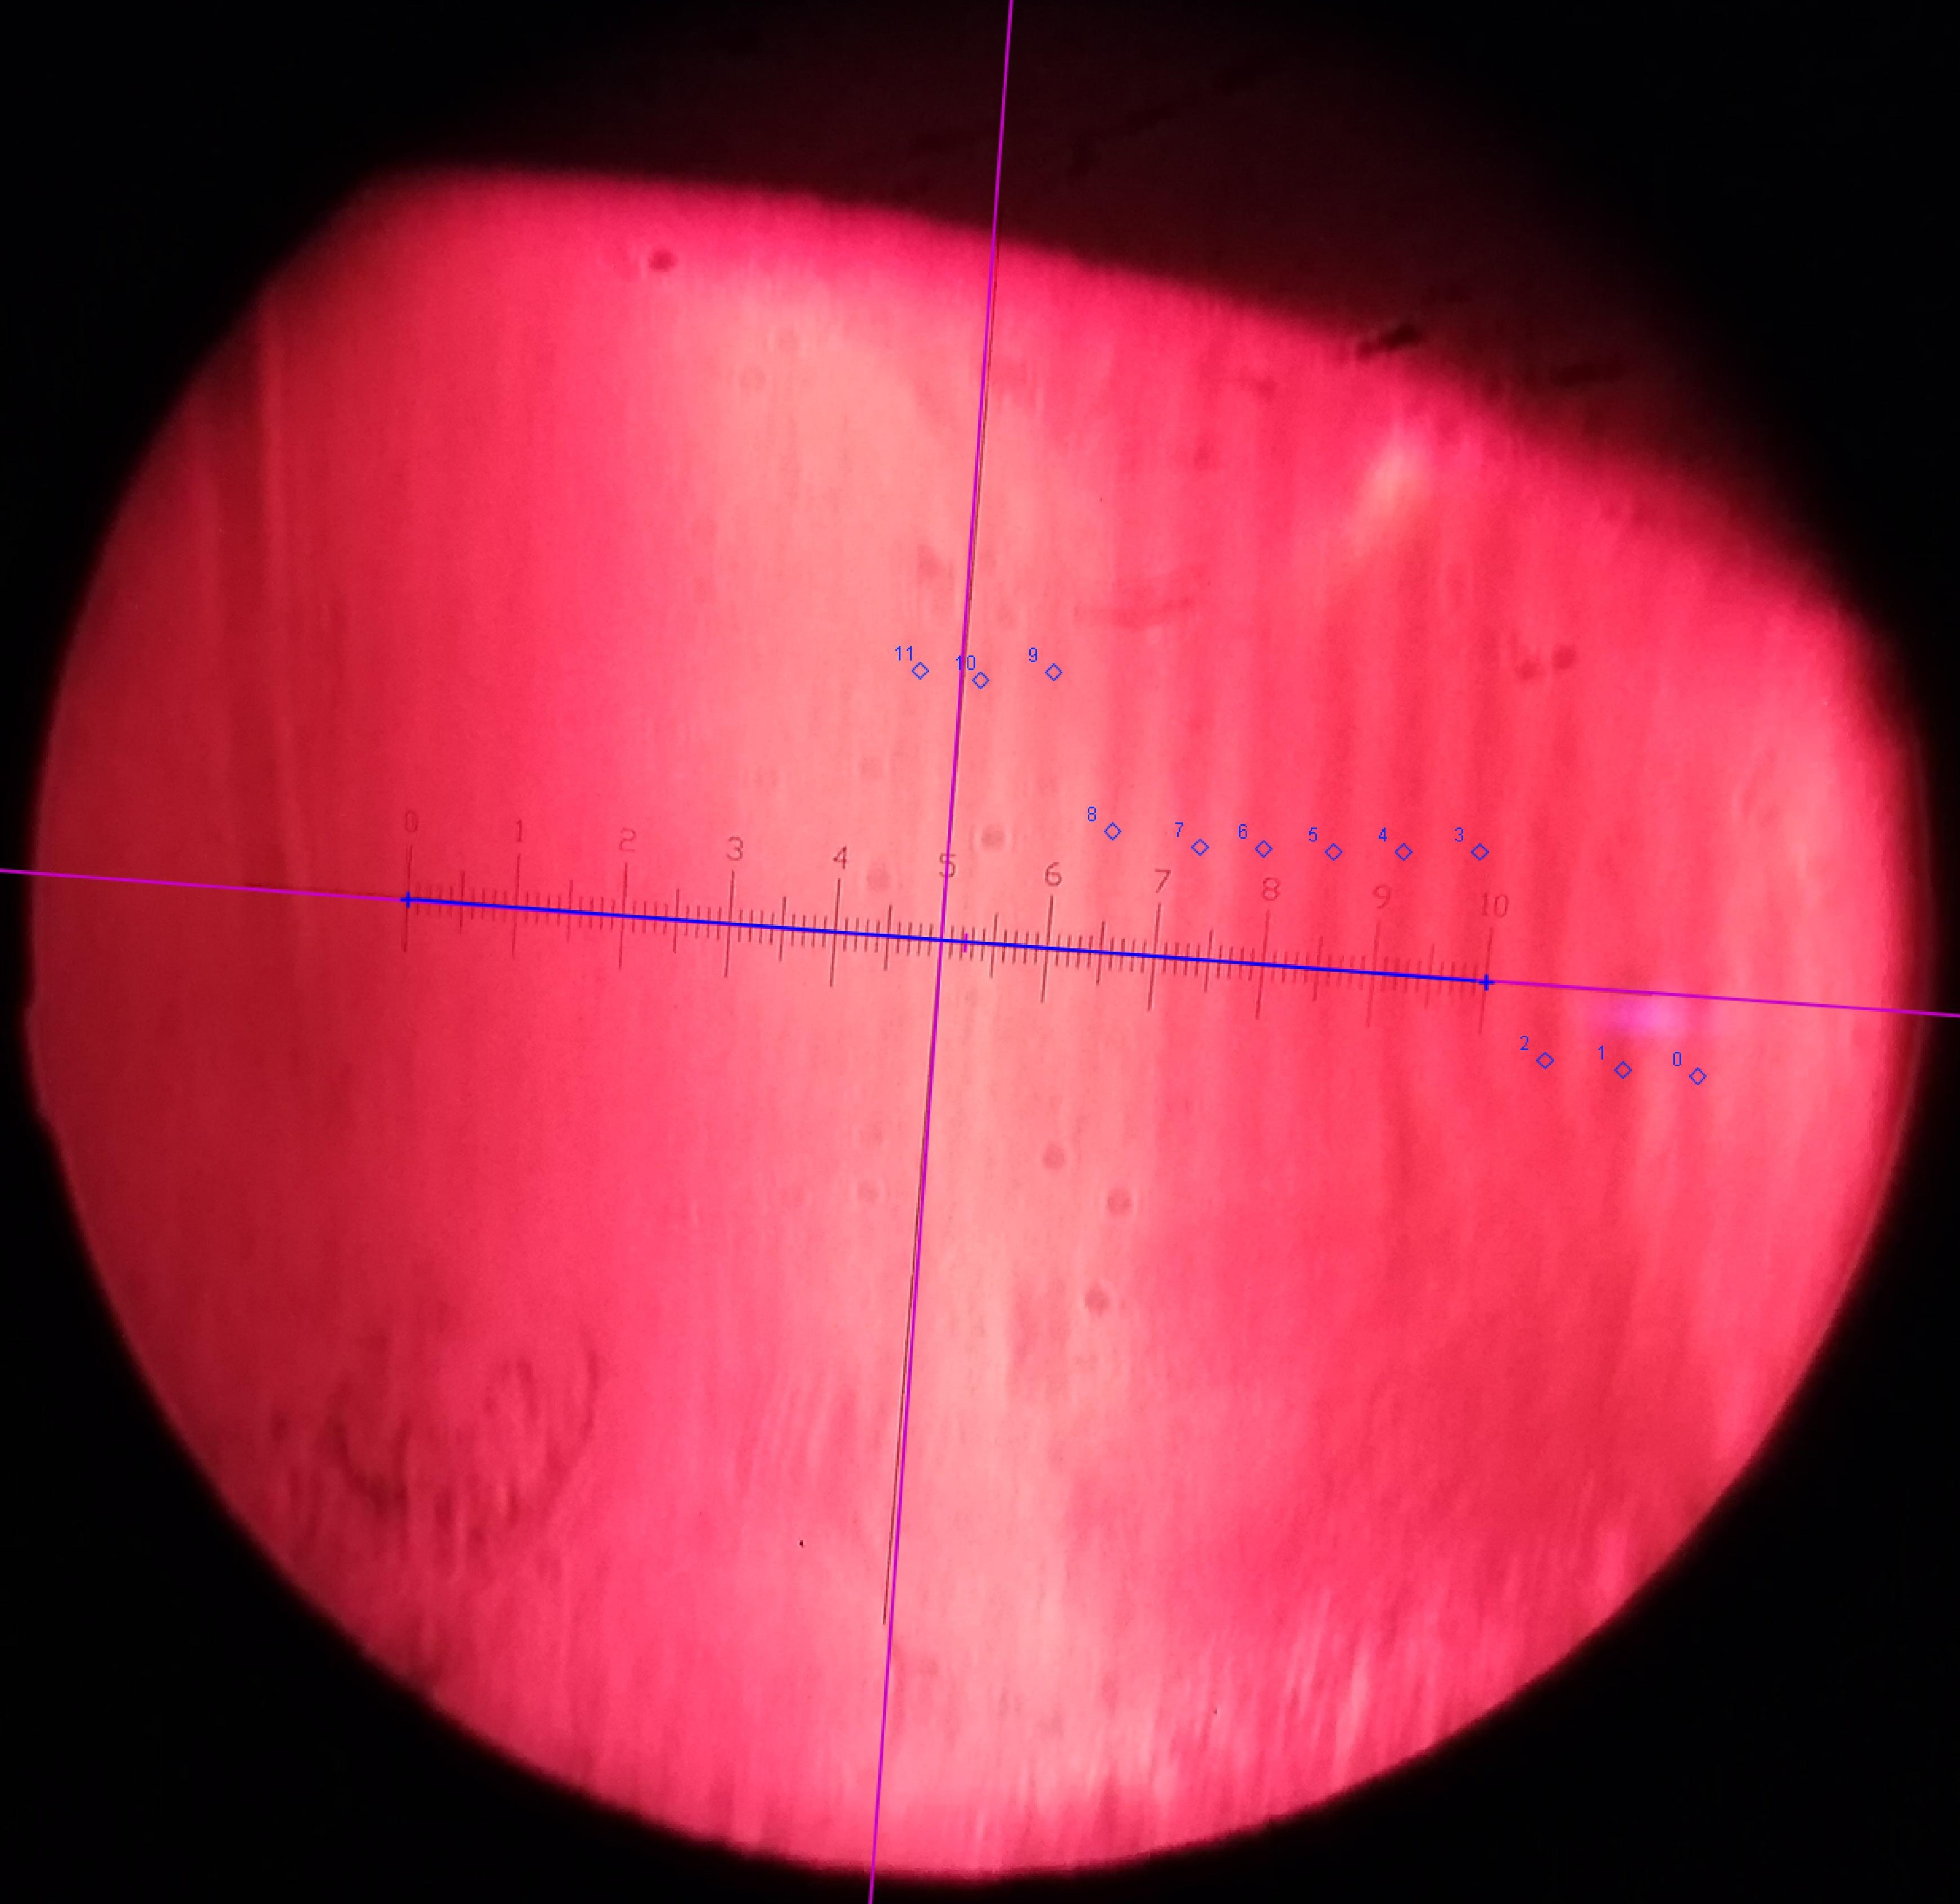
\includegraphics[height=3.5cm]{data/part2/3.jpg}
			\caption{Dark-field maxima in microscope}
		\end{figure}
		
		Picture is continuous before central maximum is cut off. When it's blocked we can observe interference pattern.
		
		Interference lines on pictures are indexed. Microscope scale is marked in blue.
		
	\end{frame}
	
	
	\begin{frame}
		\frametitle{Dark-field maxima}
		
		\begin{columns}
			\column{0.65\linewidth}
			\begin{figure}
				\includegraphics[width=1.1\linewidth]{gen/part2_xn.pdf}
				\caption{Maxima positions for different frequencies}
			\end{figure}
			\column{0.35\linewidth}
			From ($\ref{eq:dark_field}$) we obtain
			$$\Lambda = 2 \frac{x_m}{m} = 2 k.$$
			Therefore:
			$$ v = 2 k \nu.$$
			
			
			Evaluating $k$ for all frequencies and taking average:
			$$ v = (1574 \;\pm \; 12) \; \text{m/s}. $$
			
		\end{columns}
	\end{frame}

	\begin{frame}
		\frametitle{Amplitude grating}

		\begin{figure}
			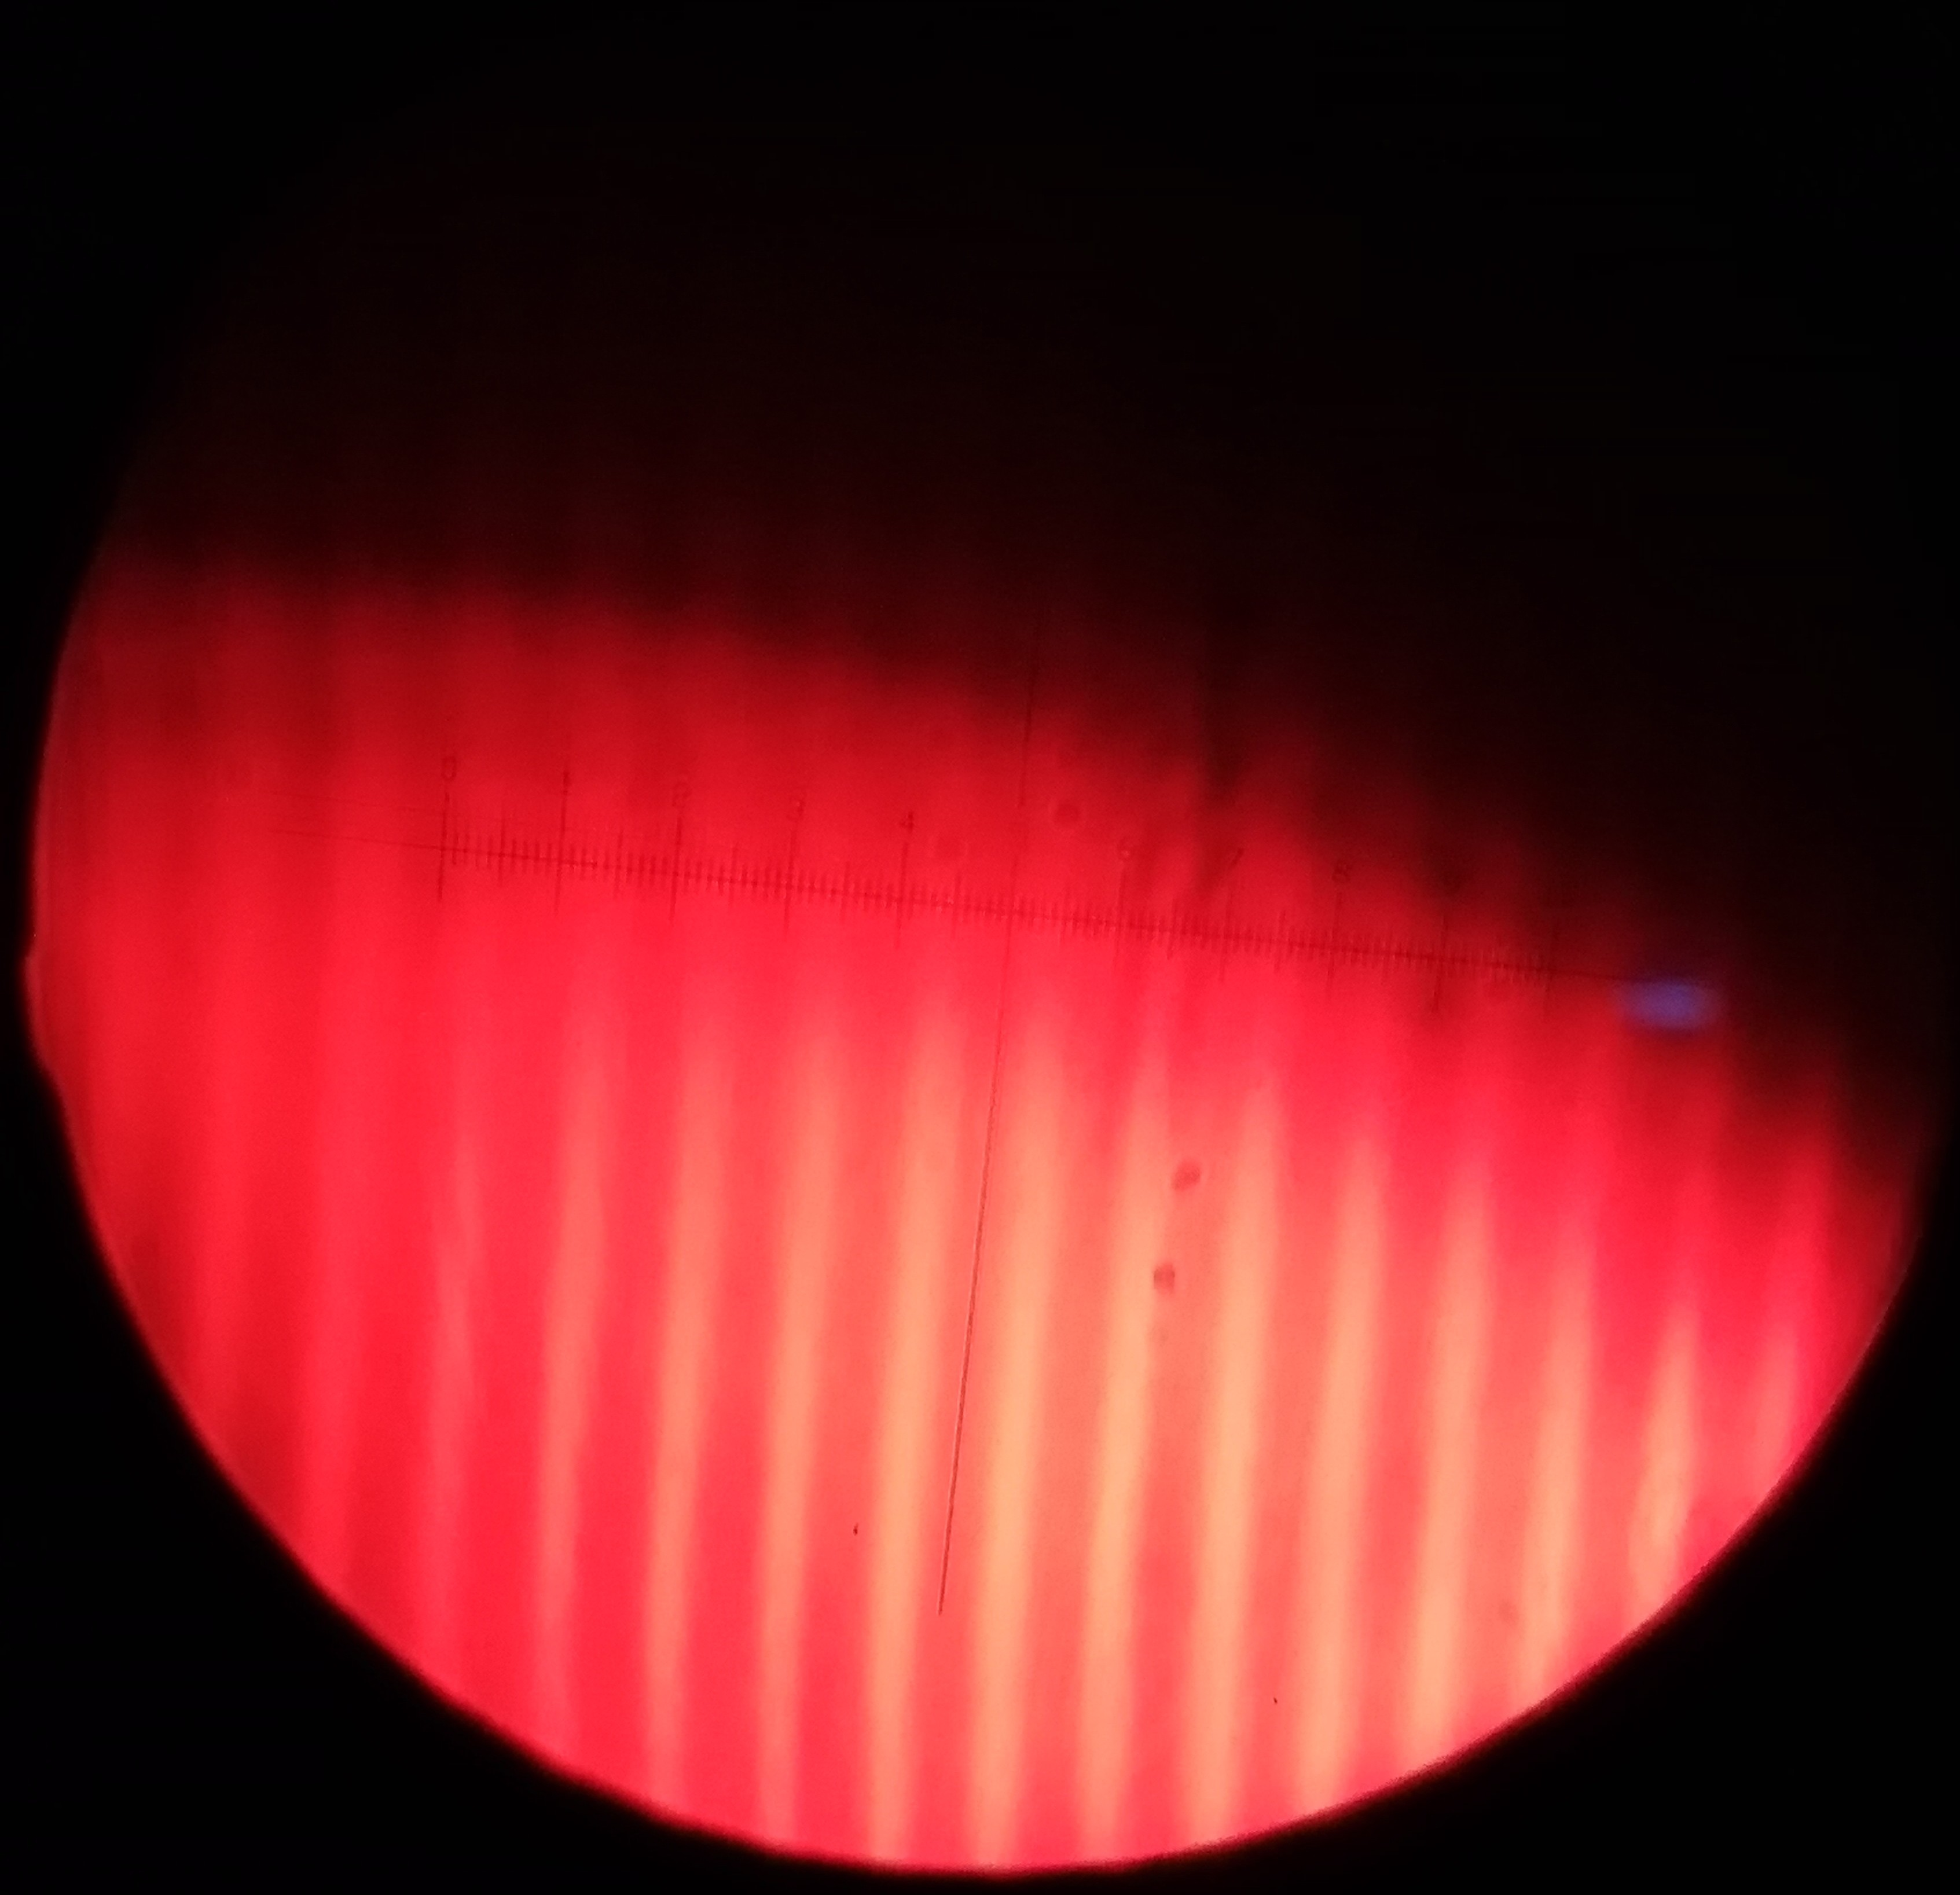
\includegraphics[width=0.3\linewidth]{data/part2/moved.jpg}
			\caption{Amplitude grating after microscope shift}
		\end{figure}
	
		We remove wire that blocks central maximum. After shifting microscope diffraction pattern appears, which is similar to pattern created by amplitude grating.
		
	\end{frame}
	
	
	
	\begin{frame}[plain,c]
		
		\begin{center}
			\huge \usebeamercolor[fg]{frametitle} Conclusion
		\end{center}
		
	\end{frame}

	\begin{frame}
		\frametitle{Conclusion}
		
		Diffraction of light by ultrasonic waves has been demonstrated. Speed of ultrasonic waves in water was obtained using two methods:
		$$ v = (1480 \pm 30) \text{ m/s -- from diffraction pattern,}$$
		$$ v = (1574 \pm 12) \text{ m/s -- from dark-field method.}$$
		
		Bulk modulus $K$ according to (\ref{eq:k}) evaluates to:
		$$ K = 2.2 \text{ GPa},$$
		$$ K = 2.5 \text{ GPa}.$$
		
		Reference values:
		$$ v = 1490 \text{ m/s},$$
		$$ K = 2.2 \text{ GPa}. $$
	\end{frame}
	
	\begin{frame}[plain,c]
		
		\begin{center}
			\huge \usebeamercolor[fg]{frametitle} Thank you for your attention!
		\end{center}
		
	\end{frame}
			
	
\end{document}